\documentclass{article}
\usepackage[main,final]{neurips_2026}
\makeatletter
\renewcommand{\@noticestring}{}
\makeatother
\usepackage[utf8]{inputenc}
\usepackage[T1]{fontenc}
\usepackage{hyperref}
\usepackage{url}
\usepackage{booktabs}
\usepackage{amsmath}
\usepackage{amsfonts}
\usepackage{graphicx}
\usepackage{microtype}
\usepackage{xcolor}
\usepackage{float}
\usepackage{caption}
\captionsetup{font=small,skip=3pt}
\setcounter{topnumber}{4}\setcounter{totalnumber}{6}\renewcommand{\topfraction}{0.9}\setlength{\textfloatsep}{8pt plus 2pt minus 2pt}
\setlength{\floatsep}{6pt plus 2pt minus 2pt}
\setlength{\intextsep}{6pt plus 2pt minus 2pt}

\title{Fine-Tuning, Visual Grounding, and\\Test-Time Compute in Small Qwen Models}
\author{Daniyal Hussain Shah}

\begin{document}
\maketitle

\begin{abstract}
This report examines three strategies for adapting and deploying pretrained models: parameter updating, visual conditioning, and inference-time computation. Task 1 fine-tunes Qwen3-0.6B on mathematics with full fine-tuning, L2-SP, LoRA at two ranks, and OPLoRA. All methods raise GSM8K by 13 to 21 points, but full fine-tuning lowers BoolQ by 6.2 points and transfers the training answer style to unrelated prompts, while LoRA and L2-SP preserve BoolQ. OPLoRA yields no measurable improvement over LoRA, and the weight-space diagnostics indicate the likely reason. Task 2 trains a SigLIP-Qwen vision-language model in three stages. Swapping in the partner image of a complementary pair lowers accuracy by 55.5 points on template questions and 24.0 points on natural questions, so answers are conditioned on the image, although pair accuracy on natural questions is only 19.8\%. Task 3 analyses supplied rollouts and live generation. Sampling raises oracle coverage to about 91\%, but selection captures only a fraction of it, and rank-weighted consensus outperforms raw confidence scores. Adaptive stopping reduces token cost by 53 to 67\% for at most 0.9 points of accuracy. Code, configurations, logs, and machine-readable results are available at \url{https://github.com/syeddaniyalg/atml-pa3}.
\end{abstract}

\section{Introduction}
Pretrained models can be adapted at several levels, and each choice carries a distinct cost. Fine-tuning can degrade previously acquired capabilities, a visual connector does not ensure that predictions are conditioned on visual evidence, and additional inference-time computation is useful only if the system can identify which candidate to trust. Task 1 compares five fine-tuning methods for mathematics, with attention to what is lost elsewhere \citep{hu2022lora,li2018l2sp,oplora,biderman2024}. Task 2 builds a SigLIP-Qwen model and tests whether its answers follow the visual evidence \citep{liu2023llava,zhai2023siglip,goyal2017vqa}. Task 3 studies sampling, answer selection, refinement, and adaptive stopping \citep{wang2023selfconsistency,kang2025selfcert,usman2025visconf,madaan2023selfrefine,aggarwal2023adaptive}. All experiments use seed 6304. Differences are in percentage points, and intervals are 95\% bootstrap intervals over examples, pairs, or questions.

\section{Task 1: Mathematical Fine-Tuning and Retention}
\subsection{Experimental Setup}
We fine-tune Qwen3-0.6B \citep{qwen3} with thinking disabled for one epoch on the first 40,000 eligible MetaMathQA examples \citep{yu2024metamath}. Training uses 1,250 updates, an effective batch of 32, AdamW, 38 warmup updates, cosine decay, and FP16 autocast with FP32 trainable parameters. The five variants are Full FT (peak learning rate $2\times10^{-5}$), Full FT with L2-SP ($\lambda=10^{-3}$), LoRA with $(r,\alpha)=(4,8)$ and $(16,32)$ at $2\times10^{-4}$ on all seven projection types, and OPLoRA with $r=16$ and protection rank $k=128$.

Evaluation uses lm-evaluation-harness \citep{gao2024harness}, zero-shot: GSM8K \citep{cobbe2021gsm8k} (flexible-extraction exact match, greedy, 1,024 new tokens), HellaSwag \citep{zellers2019hellaswag} and ARC-Easy \citep{clark2018arc} (normalized accuracy), and BoolQ \citep{clark2019boolq} (accuracy). The seven conditions are the baseline, Full FT at the midpoint (625 updates), and all five variants at the end. Intervals use a paired bootstrap over test examples (2,000 resamples). Diagnostics use \texttt{down\_proj} in layers 0, 13, and 27: the subspace interference $\rho_k$ (share of the update energy inside the top-$k$ output directions), the relative size $\eta=\|\Delta W\|_F/\|W_0\|_F$, and the response ratio $R(z)=\|\Delta W z\|_2/(\|W_0 z\|_2+10^{-8})$ on cached inputs from 32 GSM8K and 32 HellaSwag prompts.

\begin{table}[t]
\centering
\caption{Task 1 benchmark scores (\%) with change from the baseline in points. GSM8K strict match is 0.0 for every condition, and extraction is 100\%.}
\label{tab:t1-bench}
\footnotesize
\begin{tabular}{lcccc}
\toprule
Condition & GSM8K & HellaSwag & BoolQ & ARC-E \\
\midrule
Baseline & 43.59 & 47.32 & 64.37 & 56.06 \\
Full FT (midpoint) & 57.01 (+13.4) & 45.56 (-1.8) & 59.05 (-5.3) & 62.08 (+6.0) \\
Full FT & \textbf{64.75} (+21.2) & 46.04 (-1.3) & 58.13 (-6.2) & \textbf{63.59} (+7.5) \\
Full FT + L2-SP & 63.68 (+20.1) & 46.37 (-1.0) & 66.94 (+2.6) & 63.43 (+7.4) \\
LoRA-4 & 58.83 (+15.2) & 47.35 (0.0) & 70.03 (+5.7) & 62.71 (+6.7) \\
LoRA-16 & 61.79 (+18.2) & 47.28 (0.0) & 70.86 (+6.5) & 62.75 (+6.7) \\
OPLoRA-16 & 62.32 (+18.7) & 47.33 (0.0) & \textbf{70.95} (+6.6) & 62.71 (+6.7) \\
\bottomrule
\end{tabular}
\end{table}

\begin{figure}[t]
\centering
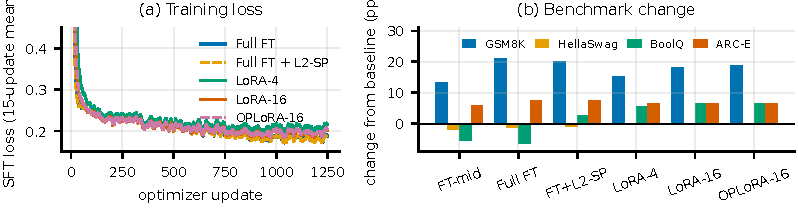
\includegraphics[width=\linewidth]{figures/task1_main.pdf}
\caption{(a) Training loss of the five runs. Full FT and Full FT + L2-SP nearly coincide, as do LoRA-16 and OPLoRA-16. (b) Change from the baseline on each benchmark (FT-mid: Full FT midpoint).}
\label{fig:t1-main}
\end{figure}

\subsection{Specialization and Retention}
Every method improves GSM8K (Table~\ref{tab:t1-bench}), from +13.4 pp for Full FT at the midpoint to +21.2 pp at the end (intervals, raw accuracy, and checkpoint sizes in Appendix~\ref{app:ci}). The gain is not an extraction artifact: extraction is 100\% everywhere and truncation stays between 0.5\% and 1.1\%. Strict match is 0 everywhere: the baseline almost never writes ``The answer is'' (1 of 1,319 responses), and the fine-tuned models write it with a colon (99\% of responses), which the stock strict pattern rejects. The flexible metric is therefore the informative one, and the colon shows that every fine-tuned model adopted the MetaMathQA answer style on math questions.

The retention cost differs by method. Full FT loses 6.2 pp on BoolQ [$-8.4,-4.2$] and 1.3 pp on HellaSwag. Most of this is already present at the midpoint (BoolQ $-5.3$, HellaSwag $-1.8$), when the model has gained 13.4 of its final 21.2 GSM8K points. The second half adds 7.7 pp on GSM8K [5.3, 10.0] and little additional forgetting. ARC-Easy rises by 6.0 to 7.5 pp for every method, including the low-rank ones. The cause was not investigated, so the increase is not interpreted as improved scientific knowledge.

\subsection{Constraints on Adaptation}
Table~\ref{tab:t1-ctrl} reports the controlled comparisons. L2-SP shrinks the final displacement $\|\theta-\theta_0\|_2$ from 10.64 to 6.27 (41\% lower) while the final SFT loss is unchanged (0.165 in both runs). The penalty $\lambda\Omega$ ends at 0.020, about 12\% of the SFT loss. The benchmark effect is one-sided: BoolQ recovers by 8.8 pp [7.5, 10.2], and GSM8K changes by $-1.1$ pp, within noise. Raising the LoRA rank from 4 to 16 quadruples the adapter (2.5M to 10.1M parameters) and lowers the final loss from 0.192 to 0.178. It raises GSM8K by 3.0 pp [0.8, 5.0] and leaves retention unchanged apart from a borderline BoolQ gain (+0.8 pp [0.0, 1.6]).

OPLoRA, with the same rank, initialization, and learning rate as LoRA-16, yields +0.5 pp GSM8K [$-1.1$, 2.1] and +0.1 pp BoolQ, so orthogonal protection yields no measurable benefit in this setting. The constraint itself holds: $\|U_k^\top \tilde B\|/\|\tilde B\|$ and $\|\tilde A V_k\|/\|\tilde A\|$ stay below $6.1\times10^{-4}$ in layers 0 and 13, and $\rho_k$ is zero to numerical precision. This verifies the implementation but provides no evidence about benchmark performance. Finally, LoRA-16 trails Full FT by 3.0 pp on GSM8K [$-5.2,-0.7$] and retains 12.7 pp more BoolQ accuracy.

\begin{table}[t]
\centering
\caption{Paired differences $a-b$ in points with 95\% intervals. Bold marks intervals that exclude zero.}
\label{tab:t1-ctrl}
\footnotesize
\begin{tabular}{llccc}
\toprule
Comparison ($a$ vs $b$) & GSM8K & HellaSwag & BoolQ & ARC-E \\
\midrule
LoRA-16 vs LoRA-4 (rank) & \textbf{+3.0 [0.8, 5.0]} & -0.1 [-0.4, 0.3] & +0.8 [0.0, 1.6] & 0.0 [-0.8, 0.9] \\
L2-SP vs Full FT (penalty) & -1.1 [-2.9, 0.8] & +0.3 [0.0, 0.7] & \textbf{+8.8 [7.5, 10.2]} & -0.2 [-1.1, 0.7] \\
OPLoRA-16 vs LoRA-16 (protection) & +0.5 [-1.1, 2.1] & 0.0 [-0.2, 0.3] & +0.1 [-0.6, 0.8] & 0.0 [-0.7, 0.6] \\
LoRA-16 vs Full FT & \textbf{-3.0 [-5.2, -0.7]} & \textbf{+1.2 [0.8, 1.8]} & \textbf{+12.7 [10.8, 14.7]} & -0.8 [-2.0, 0.3] \\
\bottomrule
\end{tabular}
\end{table}

\subsection{Weight-Space Geometry, Activation Response, and Behavior}
For Full FT, L2-SP, and both LoRA models, $\rho_k$ lies between 0.10 and 0.15 (Figure~\ref{fig:t1-diag}), close to $k/d=128/1024=0.125$, the value expected for an update distributed uniformly across output directions. The updates are therefore not concentrated in the protected subspace, which is consistent with OPLoRA's null result: protecting 128 directions intercepts only about one eighth of the update energy. The relative size $\eta$ is small for all methods (0.7\% to 1.9\%), yet the behavioral change is substantial, so update magnitude alone is not informative.

$R$ is larger on math than on non-math prompts in layers 0 and 13 for every method. For example, LoRA-4 has a median $R$ of 7.3\% on math and 1.9\% on non-math inputs in layer 13 (ratio 3.8), against 5.5\% and 3.0\% for Full FT (ratio 1.8). Full FT and L2-SP respond more strongly to non-math inputs than LoRA-4 (2.3 to 3.0\% against 1.2 to 1.9\%), which agrees with their larger BoolQ losses. The pattern is not consistent, however. LoRA-16 and OPLoRA-16 have non-math responses similar to Full FT in layers 0 and 13 but show no BoolQ loss, and in layer 27 the Full FT response is larger on non-math than on math inputs. These local measurements do not show how a change propagates through the network or establish a cause of the behavior.

\begin{figure}[t]
\centering
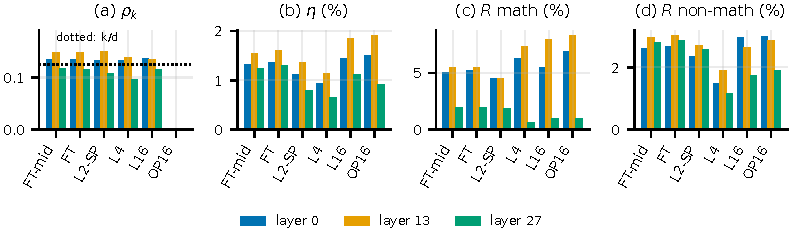
\includegraphics[width=\linewidth]{figures/task1_diag.pdf}
\caption{Diagnostics for \texttt{down\_proj} in layers 0, 13, and 27 (L4, L16: LoRA; OP16: OPLoRA-16). (a) Subspace interference, with the dotted line at $k/d$; OPLoRA is zero by construction. (b) Relative update size. (c, d) Median response ratio on math and non-math probes.}
\label{fig:t1-diag}
\end{figure}

\subsection{Computational Cost and Qualitative Behavior}
LoRA requires a peak of 3.1 to 3.3 GB against 11.7 GB for Full FT, and its adapters are 9.7 to 38.6 MB against 2,274 MB of weights (Table~\ref{tab:t1-res}). Training time is similar (2.4 to 2.7 h), because the T4 and gradient checkpointing dominate and equal updates do not mean equal compute: the LoRA runs use a ten times larger learning rate. Both Full FT variants keep a 2.2 GB CPU copy of $\theta_0$, and L2-SP spends 6.0 extra minutes on the penalty. OPLoRA stores 308 MB of bases, spends 33 s on the SVD, and trains 30\% longer than LoRA-16. LoRA-16 and OPLoRA-16 thus give the best retention for 2.4 to 3.0 pp less GSM8K than Full FT, L2-SP stays closest to Full FT on mathematics while recovering BoolQ, and Full FT is the most expensive and least balanced.

\begin{table}[t]
\centering
\caption{Resources of the five runs (one NVIDIA T4). Size is the final weights or adapter.}
\label{tab:t1-res}
\footnotesize
\begin{tabular}{lccccc}
\toprule
Method & Trainable (M) & Time (h) & Peak GPU (GB) & Size (MB) & $\|\theta-\theta_0\|_2$ \\
\midrule
Full FT & 596.05 & 2.37 & 11.69 & 2273.9 & 10.64 \\
Full FT + L2-SP & 596.05 & 2.53 & 11.69 & 2273.9 & 6.27 \\
LoRA-4 & 2.52 & 2.63 & 3.14 & 9.7 & n/a \\
LoRA-16 & 10.09 & 2.66 & 3.25 & 38.6 & n/a \\
OPLoRA-16 & 10.09 & 3.45 & 3.55 & 38.6 & n/a \\
\bottomrule
\end{tabular}
\end{table}

The 42-response subset (the first and last plain questions in three formats, seven conditions) shows effects that benchmarks miss (summary and aligned excerpts in Tables~\ref{tab:t1-qual} and~\ref{tab:t1-ex}, appendix). The baseline and the LoRA models respond in the baseline style, without truncation and with almost no math markers. Full FT at the midpoint produces a degenerate ``\#\#\#\# $n$'' pattern on the wish prompt, truncates in 3 of 6 responses, and shows heavy repetition (mean 4-gram repetition 0.32). At the end, Full FT still adds ``The answer is: 1'' to a plain question and violates the requested JSON format on both JSON prompts. L2-SP behaves like Full FT here although its BoolQ score recovered, so the penalty did not remove the stylistic transfer. OPLoRA adds one trailing ``The answer is'' and produces one off-topic repetitive reply. Benchmark retention therefore understates the change in chat behavior for the fully fine-tuned models.

\section{Task 2: A SigLIP-Qwen Vision-Language Model}
\subsection{Experimental Setup}
A frozen SigLIP base encoder \citep{zhai2023siglip} (224 pixels, 196 patch features of size 768, cached in FP16) feeds a two-layer MLP connector \citep{liu2023llava} (768 to 1024, GELU, 1024 to 1024; 1.84M parameters) whose 196 outputs are placed in the user turn before the question, with labels, masks, and positions rebuilt to match. The language model is the frozen Qwen3-0.6B. The connector output is multiplied by 0.052, chosen on 64 training captions so that its mean norm (15.96 before scaling) matches the mean text-embedding norm (0.834). From Stage 2 on, LoRA ($r=16$, $\alpha=32$) on $q,k,v,o$ adds 4.59M parameters. Data come from COCO 2014 captions \citep{lin2014coco} and VQAv2 complementary pairs \citep{goyal2017vqa}: 6,000 training images with 3 captions each, pools of 1,200 presence and 1,200 counting pairs generated from COCO instance annotations, and 1,536 natural pairs (640 yes/no, 256 number, 640 other) whose consensus answers differ and are each backed by at least 8 of 10 annotators. Development and test sets use disjoint \texttt{val2014} images: 96 captions, 24 grounding pairs, and 32 natural pairs for development, and 64 grounding pairs and 96 natural pairs for the final test. All image sets are disjoint, including from training.

Training has 2,250 caption updates (connector only, peak learning rate $10^{-3}$), 1,500 visual instruction updates (connector $10^{-4}$, LoRA $2\times10^{-5}$; draws 50\% presence, 25\% counting, 25\% caption replay), and 750 natural updates (connector $5\times10^{-5}$, LoRA $10^{-5}$; draws 70\% natural, 10\% each other source). That is 4,500 updates with batch 16, or 72,000 example presentations, and the end of Stage 3 is the final model. Evaluation uses greedy decoding with a 16-token cap under four image conditions: correct, complementary swap, mismatched (an image from another pair of the same suite, fixed before generation), and no image. Grounding questions use normalized exact match and natural questions the VQA soft score \citep{antol2015vqa}. Intervals come from 4,000 bootstrap resamples of complete pairs.

\subsection{Acquisition of the Visual Interface}
Caption alignment lowers the dev caption loss from 5.47 to 2.19, and later stages leave it unchanged (2.18 at the end), so caption replay prevented forgetting (Figure~\ref{fig:t2-dev}; training loss and answer NLL in Appendix~\ref{app:t2}). After Stage 1 the model has an interface but cannot answer questions: dev accuracy is 8.3\% on grounding and 12.3\% on natural questions, and the swap penalty $\Delta_{\mathrm{NLL}}$ is only 0.10 and 0.32. Question answering emerges in Stage 2. At update 2,500 accuracy is 68.8\% and 52.7\%, the grounding answer NLL falls from 4.88 to 0.73, and the grounding penalty rises to 2.79 and then to a peak of 5.29 at update 3,750. Stage 3 lowers the grounding penalty to 3.13 with accuracy staying near 69\%. The natural penalty falls from 1.33 to 0.67, while natural dev accuracy rises from 50.6\% to 55.3\% and its NLL falls from 1.92 to 1.20. Natural questions have only 32 dev pairs, so differences of a few points are within sampling noise.

\begin{figure}[t]
\centering
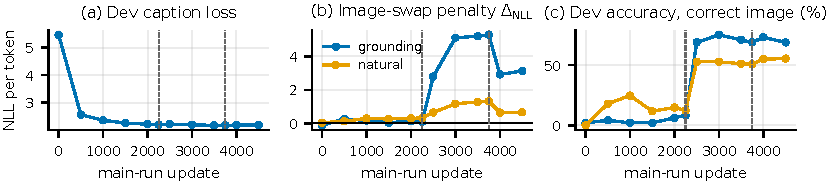
\includegraphics[width=\linewidth]{figures/task2_dev.pdf}
\caption{Development metrics for the 196-token model. Dashed lines mark stage boundaries (updates 2,250 and 3,750). $\Delta_{\mathrm{NLL}}$ is the answer NLL under the partner image minus that under the correct image.}
\label{fig:t2-dev}
\end{figure}

\subsection{Visual Grounding and Image Dependence}
With the correct image the model reaches 71.1\% on the grounding suite (presence 93.8\%, counting 48.4\%) and 54.2\% on natural questions (yes/no 59.2\%, number 62.3\%, other 43.8\%; Table~\ref{tab:t2-final}). A swap lowers accuracy to 15.6\% and 30.2\%, an advantage of the correct image of 55.5 pp [41.4, 69.5] and 24.0 pp [15.3, 32.9]. The answer NLL moves the same way (+3.03 [2.37, 3.69] and +1.02 [0.68, 1.41]). Under a swap, 71.1\% of grounding predictions and 51.0\% of natural predictions equal the partner image's answer, against 15.6\% and 27.1\% with the correct image, so predictions are conditioned on the image rather than produced from the question alone.

The two suites differ in the strength of this dependence. On grounding, presence falls to 6.2\% under a swap, and counting to 25.0\%. With no image, presence is exactly 50\% because the model always answers ``no'', so counting (48.4\% falling to 15.6\%) is the clearer evidence of image use. On natural questions, language priors carry much of the yes/no accuracy (48.6\% without an image against 59.2\%), and ``other'' falls from 43.8\% to 16.9\%. A mismatched image behaves almost like no image (32.7\% and 30.6\% on natural questions).

The measures agree in direction but differ in magnitude. Pair accuracy is far below per-answer accuracy (56.2\% on grounding, 19.8\% on natural), since both answers must be right. On natural questions the two images of a pair receive the same answer in 56.2\% of cases, and since the references of a pair differ by construction, at least one of these answers is wrong. A large part of the natural-question behavior therefore remains consistent with a language prior, even though NLL favors the correct image. The grounding dev swap penalty also fell from 5.29 to 2.93 between updates 3,750 and 4,000 while dev accuracy stayed between 69 and 73\%, so likelihood and generated accuracy are different measurements. Question-type results, empty-answer rates, generation times, and examples are in Appendix~\ref{app:t2}.

\begin{table}[t]
\centering
\caption{Final test results for the 196-token model, with 95\% pair-bootstrap intervals for accuracy. Pair: both answers of a pair correct (\%). Same: the two answers of a pair are identical (\%). NLL: reference-answer NLL without the end token.}
\label{tab:t2-final}
\footnotesize
\setlength{\tabcolsep}{3pt}
\begin{tabular}{lcccc@{\hspace{9pt}}cccc}
\toprule
 & \multicolumn{4}{c}{Grounding (64 pairs)} & \multicolumn{4}{c}{Natural (96 pairs)} \\
\cmidrule(lr){2-5}\cmidrule(lr){6-9}
Image & Acc. (\%) & Pair & Same & NLL & Acc. (\%) & Pair & Same & NLL \\
\midrule
Correct & 71.1 [62.5, 79.7] & 56.2 & 21.9 & 0.85 & 54.2 [48.1, 60.3] & 19.8 & 56.2 & 1.42 \\
Swap & 15.6 [9.4, 21.9] & 3.1 & 21.9 & 3.88 & 30.2 [24.3, 36.1] & 3.1 & 56.2 & 2.44 \\
Mismatched & 35.2 [28.1, 42.2] & 6.2 & 59.4 & 2.58 & 32.7 [27.2, 38.5] & 4.2 & 49.0 & 2.25 \\
No image & 32.8 [27.3, 38.3] & 0.0 & 100 & 2.04 & 30.6 [25.2, 35.9] & 0.0 & 100 & 2.46 \\
\bottomrule
\end{tabular}
\end{table}

\subsection{Capabilities and Computational Cost}
Trainable parameters are 1.84M in Stage 1 and 6.42M in Stages 2 and 3, against about 0.6B frozen language-model parameters. The three stages take 45.0, 33.3, and 16.8 minutes (95 minutes in total) with peak GPU memory of 1.89, 1.95, and 1.95 GB on one T4, excluding development evaluation. The feature cache for 9,283 images adds 5.5 minutes, 0.43 GB, and 2.67 GB of storage, and final evaluation of both suites under four conditions takes 1.2 minutes (0.04 s per answer). The optional 49-token model (2$\times$2 pooling) reaches 68.8\% [59.4, 77.3] on grounding and 47.6\% [40.4, 54.8] on natural questions. The intervals overlap those of the 196-token model, so the loss is not established, but the natural swap advantage falls from 24.0 to 16.6 pp. Training time falls by 44\% (3,218 s against 5,701 s) and peak memory from 1.95 to 1.49 GB (Appendix~\ref{app:t2}).

\section{Task 3: Sampling, Selection, and Adaptive Inference}
\subsection{Experimental Setup}
We use the supplied 32 rollouts per question from Qwen2.5-3B-Instruct \citep{qwen25} on MATH \citep{hendrycks2021math} and Qwen2.5-VL-3B-Instruct \citep{qwen25vl} on MathVista \citep{lu2024mathvista}. In each dataset the 1,000 sorted question IDs are permuted with \texttt{default\_rng(6304)}: the first 200 are the development set and the other 800 the held-out set. Ten seeded permutations of the 32 rollouts set the reveal order, shared by all methods. MATH answers are grouped and graded with Math-Verify \citep{mathverify} (version 0.9.0), and MathVista answers use option letters and the answer-type and precision rules from the question metadata. Missing extractions form one NO\_ANSWER group that is always incorrect but still counts in voting and cost (1.6\% of MATH and 9.5\% of MathVista rollouts). Ties go to the earliest rollout. Cost is the sum of retained token counts of the consumed candidates. We compare FirstAns, self-consistency (SC), highest mean log-probability, highest self-certainty, and rank-weighted consensus (RWC), and for MathVista also vision engagement and VisConf, each with highest-score selection and with RWC. Intervals use 1,000 paired question-level bootstrap resamples after averaging over orders.

\subsection{Candidate Coverage versus Selection Quality}
Oracle coverage rises from 64.4\% to 91.4\% on MATH and from 54.5\% to 90.4\% on MathVista between $N=1$ and $N=32$, and the number of distinct answer groups grows from 1.0 to 5.9 and 4.4 (Figure~\ref{fig:t3-curves}). Even the best method recovers only part of this headroom: at $N=32$ the gap to coverage is 15.7 pp on MATH (91.4 against 75.7) and 25.6 pp on MathVista (90.4 against 64.8). The failures change with $N$. Questions with no correct candidate shrink from 35.6\% to 8.6\% (MATH) and from 45.5\% to 9.6\% (MathVista), while questions where a correct candidate existed but SC missed it grow from 0 to 17.5\% and 26.4\%. Additional samples therefore mainly contribute alternatives that the selector must identify, and this identification is the limiting step.

Signal and aggregation play different roles (Table~\ref{tab:t3-methods}). Mean log-probability is an unreliable selector and degrades as $N$ grows (MathVista 54.5\% to 49.0\%, $-5.5$ pp against FirstAns [$-7.9,-2.8$]). Within questions its top rollouts are only 2.5 pp more often correct than its bottom rollouts on MathVista, and shortest-rollout selection (62.6\% on MATH) is about as good as it (64.1\%), so length explains part of it (Appendix~\ref{app:t3}). Self-certainty helps on MATH (70.8\%, +6.3 pp over FirstAns) but not on MathVista (55.6\%, +1.1 pp [$-1.4$, 3.8]). Vision engagement alone provides no gain (54.2\%), and VisConf reaches 58.5\% (+4.0 pp [1.3, 6.5]). Aggregation matters more than the score: RWC raises self-certainty by 4.9 pp on MATH [2.9, 7.2] and 9.0 pp on MathVista [6.1, 12.0], vision by 9.9 pp, and VisConf by 6.3 pp, bringing all of them close to SC. Over SC the gain is small: +1.8 pp for self-certainty RWC on MATH [0.7, 3.0], and +0.8 pp for VisConf RWC on MathVista [$-0.7$, 2.4], which is not significant. VisConf RWC and self-certainty RWC differ by 0.1 pp on MathVista [$-1.1$, 1.4], so there is no evidence that the visual signal improves the final selection.

Confidence and visual attention are negatively associated. Across held-out MathVista rollouts the mean within-rollout correlation between calibrated confidence $c_t$ and visual engagement $v_t$ is $-0.21$, negative in 89\% of questions (Figure~\ref{fig:t3-adaptive}c), indicating that confident tokens tend to allocate less attention to the image. Combining the signals at each token instead of per rollout changes the score only by the covariance term (checked to $2\times10^{-10}$) and does not help: it lowers VisConf by 1.6 pp [$-3.5$, 0.3] with highest-score selection and by 0.3 pp [$-1.0$, 0.4] with RWC. In the three illustrative cases of Appendix~\ref{app:t3}, the highest-VisConf rollout is also the shortest, and engagement decays with token position, so part of VisConf may reflect rollout length. These associations describe how the signals co-vary and do not establish causal visual grounding.

\begin{figure}[t]
\centering
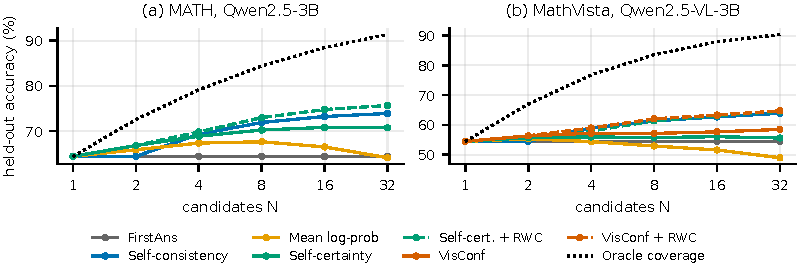
\includegraphics[width=\linewidth]{figures/task3_curves.pdf}
\caption{Held-out accuracy against the number of candidates (RWC dashed). The dotted line is oracle coverage. FirstAns uses one candidate at every $N$.}
\label{fig:t3-curves}
\end{figure}

\begin{table}[t]
\centering
\caption{Held-out accuracy (\%) at $N=8$ and $N=32$. Mean token cost at $N=32$ is 21,347 (MATH) and 8,898 (MathVista); FirstAns costs one rollout (670 and 278). n/a means the method needs images.}
\label{tab:t3-methods}
\footnotesize
\begin{tabular}{lcccc}
\toprule
 & \multicolumn{2}{c}{MATH} & \multicolumn{2}{c}{MathVista} \\
\cmidrule(lr){2-3}\cmidrule(lr){4-5}
Method & $N=8$ & $N=32$ & $N=8$ & $N=32$ \\
\midrule
FirstAns & 64.4 & 64.4 & 54.5 & 54.5 \\
Self-consistency & 71.9 & 73.9 & 61.4 & 63.9 \\
Mean log-probability & 67.6 & 64.1 & 52.9 & 49.0 \\
Self-certainty & 70.2 & 70.8 & 55.8 & 55.6 \\
Self-certainty + RWC & \textbf{73.0} & \textbf{75.7} & 61.4 & 64.6 \\
Vision engagement & n/a & n/a & 55.0 & 54.2 \\
Vision + RWC & n/a & n/a & 61.1 & 64.1 \\
VisConf & n/a & n/a & 57.2 & 58.5 \\
VisConf + RWC & n/a & n/a & \textbf{62.0} & \textbf{64.8} \\
VisConf, token-wise + RWC & n/a & n/a & 62.2 & 64.5 \\
\bottomrule
\end{tabular}
\end{table}

\subsection{Parallel Sampling versus Sequential Refinement}
On the fixed 50 MATH questions (FP16, 3,072-token allowance), a single long response, three parallel 1,024-token responses with SC, and one 1,024-token response followed by a 2,048-token review \citep{madaan2023selfrefine} reach 58\%, 58\%, and 62\% accuracy (Table~\ref{tab:t3-live}). No difference is significant: refinement minus long is +4 pp [$-6$, 16], parallel minus long is 0 [$-14$, 12], and refinement minus parallel is +4 [$-4$, 12]. The realized costs differ more than the nominal allowances suggest. Parallel sampling generates 1,840 output tokens per question, 2.4 times the long response (760), and takes 88 s against 40 s. Its 1,024-token cap truncates 14.7\% of responses (long: 4\%) and leaves 85\% of answers extractable (long: 96\%). Refinement has complete extraction, 1,229 output and 877 input tokens, and 60 s. The review changed the answer in 11 of 50 questions, fixing 2 wrong answers (initial accuracy 60\%) and breaking 1 correct answer. Both wrong-to-correct cases had an initial response truncated at 1,024 tokens without a boxed answer, so the gain reflects repair of truncation, and the one correct-to-wrong case changed $3/16$ to $3/32$ (Appendix~\ref{app:t3}). With 50 questions we cannot separate these effects from chance.

\begin{table}[t]
\centering
\caption{Live MATH comparison on 50 questions (batch size 1, peak GPU memory 5.9 GB for all). Time excludes model loading; truncation is per response.}
\label{tab:t3-live}
\footnotesize
\begin{tabular}{lccccc}
\toprule
Strategy & Accuracy (\%) & Input / output tokens & Seconds & Truncated (\%) & Extracted (\%) \\
\midrule
Single long response & 58 & 108 / 760 & 40 & 4.0 & 96 \\
Parallel (3 $\times$ 1,024) + SC & 58 & 325 / 1,840 & 88 & 14.7 & 85 \\
Refinement (1,024 + 2,048) & 62 & 877 / 1,229 & 60 & 9.0 & 100 \\
\bottomrule
\end{tabular}
\end{table}

\subsection{Adaptive Stopping}
We simulate stopping after $n\in\{4,8,16\}$ candidates \citep{aggarwal2023adaptive} and return the SC answer. The agreement rule stops when a unique non-NO\_ANSWER answer has support of at least $\tau$. The quality-aware rule also needs the RWC winner to agree with SC and an RWC margin of at least $\gamma$ (self-certainty for MATH, VisConf for MathVista). Settings were chosen on the development set as the cheapest one within 1 pp of fixed-32 SC, with ties broken by higher accuracy and then smaller $\tau$ and $\gamma$, and were frozen before held-out evaluation (Table~\ref{tab:t3-adapt}). The chosen margin is $\gamma=0$ in both datasets, so the margin condition contributed nothing beyond requiring the two winners to agree.

On held-out questions, agreement matches fixed-32 on MATH (73.8\% against 73.9\%) with 53\% fewer tokens, and the quality-aware rule loses 0.6 pp [$-1.2$, $-0.1$] with 64\% fewer. On MathVista, agreement is 0.9 pp lower [$-2.0$, 0.2] with 67\% fewer tokens and the quality-aware rule 0.5 pp lower [$-1.5$, 0.4] with 63\% fewer. At similar cost the adaptive policies sit above the fixed-$N$ curve (Figure~\ref{fig:t3-adaptive}a,b): on MATH, agreement reaches 73.8\% at 10.1k tokens against 73.2\% for $N=16$ at 10.7k, and the quality-aware rule 73.3\% at 7.7k against 71.9\% for $N=8$ at 5.3k. Most questions stop at $N=4$ (66\% and 76\% on MATH under the two rules, 76\% and 70\% on MathVista), and these are predominantly easy questions: those whose pool is at least two-thirds correct reach 99.5 to 99.9\% accuracy with about 4.1 to 4.4 rollouts.

Premature stops fail when the early majority is incorrect. Under agreement, 88.9\% (MATH) and 70.0\% (MathVista) of early stops are correct, and incorrect early stops make up 8.1\% and 25.9\% of all cases. Only 0.6\% and 4.1\% of cases would have been rescued by fixed-32 SC, so a consistent but incorrect early consensus is the dominant failure mode, which a few additional samples would not correct. The illustrative cases in Appendix~\ref{app:t3} show the same pattern: ties between equally supported answers are resolved by rollout order, and early majorities of three of four candidates are not supported by the full pool. Questions with an intermediate share of correct candidates (0.34 to 0.67) lose accuracy (MathVista 71.3\% against 81.7\% for fixed-32), and questions with fewer than a third correct stay near 10\% under any policy. These are offline simulations, and the token cost excludes prefill, attention collection, and scoring.

\begin{table}[t]
\centering
\caption{Held-out adaptive sampling. $\Delta$ is the accuracy difference to fixed-32 SC with a paired 95\% interval. Tokens are mean generated tokens per question. The last column is the share of questions stopping at $N=4,8,16,32$ (\%).}
\label{tab:t3-adapt}
\footnotesize
\setlength{\tabcolsep}{4pt}
\begin{tabular}{llcccccc}
\toprule
Data & Policy (dev-selected) & Acc. (\%) & Tokens & Rollouts & $\Delta$ (pp) & Stops \\
\midrule
MATH & Fixed-32 SC & 73.9 & 21,347 & 32.0 & n/a & 0/0/0/100 \\
 & Agreement ($\tau=0.625$) & 73.8 & 10,137 & 11.8 & -0.15 [-0.50, 0.15] & 66/6/1/27 \\
 & Quality ($\tau=0.5,\gamma=0$) & 73.3 & 7,663 & 9.0 & -0.61 [-1.18, -0.09] & 76/6/1/16 \\
\midrule
MathVista & Fixed-32 SC & 63.9 & 8,898 & 32.0 & n/a & 0/0/0/100 \\
 & Agreement ($\tau=0.5$) & 63.0 & 2,919 & 8.4 & -0.90 [-1.97, 0.21] & 76/8/2/14 \\
 & Quality ($\tau=0.5,\gamma=0$) & 63.4 & 3,280 & 9.6 & -0.53 [-1.50, 0.44] & 70/10/3/17 \\
\bottomrule
\end{tabular}
\end{table}

\begin{figure}[t]
\centering
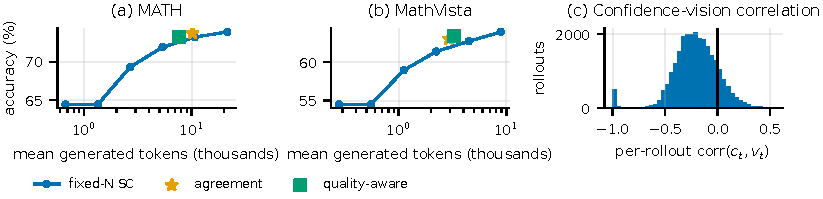
\includegraphics[width=\linewidth]{figures/task3_adaptive.pdf}
\caption{(a, b) Held-out accuracy against mean generated tokens for fixed-$N$ SC and the adaptive policies. (c) Correlation between calibrated confidence and visual engagement within held-out MathVista rollouts.}
\label{fig:t3-adaptive}
\end{figure}

\section{Conclusion}
In Task 1, every method raised GSM8K by 13 to 21 points, and the retention cost depended on how the update was restricted. Full FT lost 6.2 points of BoolQ and changed chat style, L2-SP recovered BoolQ for a 1.1-point GSM8K cost that we cannot distinguish from zero, and LoRA preserved retention at a cost of 3.0 GSM8K points relative to Full FT. OPLoRA provided no measurable benefit. In Task 2, the curriculum produced answers that depend on the image (drops of 55.5 and 24.0 points under a swap), but natural pair accuracy is 19.8\% and many answers still follow language priors. In Task 3, additional samples raise coverage considerably more than accuracy, consensus is the most reliable selection signal, and adaptive stopping saves half to two thirds of the tokens for under one point of accuracy. The main limitations are single-seed comparisons, small test sets, local diagnostics on one matrix type, an unexplained ARC-Easy gain, and the confounding of vision with model and dataset in Task 3.

\small
\begin{thebibliography}{30}
\bibitem[Aggarwal et~al.(2023)]{aggarwal2023adaptive}
Pranjal Aggarwal, Aman Madaan, Yiming Yang, and Mausam. Let's sample step by step: Adaptive-Consistency for efficient reasoning and coding with LLMs. In \emph{EMNLP}, 2023.
\bibitem[Antol et~al.(2015)]{antol2015vqa}
Stanislaw Antol, Aishwarya Agrawal, Jiasen Lu, et~al. VQA: Visual question answering. In \emph{ICCV}, 2015.
\bibitem[Bai et~al.(2025)]{qwen25vl}
Shuai Bai, Keqin Chen, Xuejing Liu, et~al. Qwen2.5-VL technical report. \emph{arXiv:2502.13923}, 2025.
\bibitem[Biderman et~al.(2024)]{biderman2024}
Dan Biderman, Jacob Portes, Jose~Javier Gonzalez~Ortiz, et~al. LoRA learns less and forgets less. \emph{Transactions on Machine Learning Research}, 2024.
\bibitem[Clark et~al.(2018)]{clark2018arc}
Peter Clark, Isaac Cowhey, Oren Etzioni, et~al. Think you have solved question answering? Try ARC, the AI2 reasoning challenge. \emph{arXiv:1803.05457}, 2018.
\bibitem[Clark et~al.(2019)]{clark2019boolq}
Christopher Clark, Kenton Lee, Ming-Wei Chang, Tom Kwiatkowski, Michael Collins, and Kristina Toutanova. BoolQ: Exploring the surprising difficulty of natural yes/no questions. In \emph{NAACL}, 2019.
\bibitem[Cobbe et~al.(2021)]{cobbe2021gsm8k}
Karl Cobbe, Vineet Kosaraju, Mohammad Bavarian, et~al. Training verifiers to solve math word problems. \emph{arXiv:2110.14168}, 2021.
\bibitem[Gao et~al.(2024)]{gao2024harness}
Leo Gao, Jonathan Tow, Baber Abbasi, et~al. A framework for few-shot language model evaluation. Zenodo, 2024.
\bibitem[Goyal et~al.(2017)]{goyal2017vqa}
Yash Goyal, Tejas Khot, Douglas Summers-Stay, Dhruv Batra, and Devi Parikh. Making the V in VQA matter: Elevating the role of image understanding in visual question answering. In \emph{CVPR}, 2017.
\bibitem[Hendrycks et~al.(2021)]{hendrycks2021math}
Dan Hendrycks, Collin Burns, Saurav Kadavath, et~al. Measuring mathematical problem solving with the MATH dataset. In \emph{NeurIPS Datasets and Benchmarks}, 2021.
\bibitem[Hu et~al.(2022)]{hu2022lora}
Edward Hu, Yelong Shen, Phillip Wallis, et~al. LoRA: Low-rank adaptation of large language models. In \emph{ICLR}, 2022.
\bibitem[Kang et~al.(2025)]{kang2025selfcert}
Zhewei Kang, Xuandong Zhao, and Dawn Song. Scalable best-of-N selection for large language models via self-certainty. \emph{arXiv}, 2025.
\bibitem[Kydl{\'i}{\v{c}}ek(2025)]{mathverify}
Hynek Kydl{\'i}{\v{c}}ek. Math-Verify: A robust mathematical expression evaluation system. Hugging Face, 2025.
\bibitem[Li et~al.(2018)]{li2018l2sp}
Xuhong Li, Yves Grandvalet, and Franck Davoine. Explicit inductive bias for transfer learning with convolutional networks. In \emph{ICML}, 2018.
\bibitem[Lin et~al.(2014)]{lin2014coco}
Tsung-Yi Lin, Michael Maire, Serge Belongie, et~al. Microsoft COCO: Common objects in context. In \emph{ECCV}, 2014.
\bibitem[Liu et~al.(2023)]{liu2023llava}
Haotian Liu, Chunyuan Li, Qingyang Wu, and Yong~Jae Lee. Visual instruction tuning. In \emph{NeurIPS}, 2023.
\bibitem[Madaan et~al.(2023)]{madaan2023selfrefine}
Aman Madaan, Niket Tandon, Prakhar Gupta, et~al. Self-Refine: Iterative refinement with self-feedback. In \emph{NeurIPS}, 2023.
\bibitem[Lu et~al.(2024)]{lu2024mathvista}
Pan Lu, Hritik Bansal, Tony Xia, et~al. MathVista: Evaluating mathematical reasoning of foundation models in visual contexts. In \emph{ICLR}, 2024.
\bibitem[Xiong and Xie(2025)]{oplora}
Yifeng Xiong and Xiaohui Xie. OPLoRA: Orthogonal projection LoRA prevents catastrophic forgetting during parameter-efficient fine-tuning. \emph{arXiv}, 2025.
\bibitem[Usman et~al.(2025)]{usman2025visconf}
Usman et~al. VisConf: Quality-aware consensus for best-of-N in vision-language model reasoning. \emph{arXiv}, 2025.
\bibitem[Wang et~al.(2023)]{wang2023selfconsistency}
Xuezhi Wang, Jason Wei, Dale Schuurmans, et~al. Self-consistency improves chain of thought reasoning in language models. In \emph{ICLR}, 2023.
\bibitem[Qwen Team(2024)]{qwen25}
Qwen Team. Qwen2.5 technical report. \emph{arXiv:2412.15115}, 2024.
\bibitem[Yang et~al.(2025)]{qwen3}
An~Yang, Anfeng Li, Baosong Yang, et~al. Qwen3 technical report. \emph{arXiv:2505.09388}, 2025.
\bibitem[Yu et~al.(2024)]{yu2024metamath}
Longhui Yu, Weisen Jiang, Han Shi, et~al. MetaMath: Bootstrap your own mathematical questions for large language models. In \emph{ICLR}, 2024.
\bibitem[Zellers et~al.(2019)]{zellers2019hellaswag}
Rowan Zellers, Ari Holtzman, Yonatan Bisk, Ali Farhadi, and Yejin Choi. HellaSwag: Can a machine really finish your sentence? In \emph{ACL}, 2019.
\bibitem[Zhai et~al.(2023)]{zhai2023siglip}
Xiaohua Zhai, Basil Mustafa, Alexander Kolesnikov, and Lucas Beyer. Sigmoid loss for language image pre-training. In \emph{ICCV}, 2023.
\end{thebibliography}

\normalsize
\appendix
\section{Supplementary Results for Task 1}
\label{app:ci}
Table~\ref{tab:app-ci} lists the paired differences of each condition from the baseline with 95\% intervals (2,000 resamples over test examples; saved in \texttt{results/task1/tables/bootstrap\_ci.csv}). The data statistics were: 40,002 examples scanned, 40,000 kept, 2 too long, 0 empty, 0 overlapping with GSM8K. The gradient scaler skipped no update in any Task 1 run. Merged and unmerged logits agreed on the argmax at 99.7\% (LoRA-4), 99.9\% (LoRA-16), and 100\% (OPLoRA-16) of positions, with maximum absolute logit differences of 0.15 to 0.22, consistent with FP16 rounding.

\begin{table}[H]
\centering
\caption{Change from the baseline in points with 95\% intervals (Task 1). Bold means the interval excludes zero.}
\label{tab:app-ci}
\footnotesize
\begin{tabular}{lcccc}
\toprule
Condition & GSM8K & HellaSwag & BoolQ & ARC-E \\
\midrule
Full FT (midpoint) & \textbf{+13.4 [10.2, 16.8]} & \textbf{-1.8 [-2.4, -1.2]} & \textbf{-5.3 [-7.5, -3.2]} & \textbf{+6.0 [4.5, 7.6]} \\
Full FT & \textbf{+21.2 [18.0, 24.2]} & \textbf{-1.3 [-1.9, -0.7]} & \textbf{-6.2 [-8.4, -4.2]} & \textbf{+7.5 [6.0, 9.1]} \\
Full FT + L2-SP & \textbf{+20.1 [17.1, 23.2]} & \textbf{-1.0 [-1.5, -0.4]} & \textbf{+2.6 [0.6, 4.4]} & \textbf{+7.4 [5.9, 8.9]} \\
LoRA-4 & \textbf{+15.2 [12.1, 18.4]} & 0.0 [-0.4, 0.5] & \textbf{+5.7 [3.9, 7.4]} & \textbf{+6.7 [5.2, 8.1]} \\
LoRA-16 & \textbf{+18.2 [15.1, 21.3]} & 0.0 [-0.5, 0.4] & \textbf{+6.5 [4.7, 8.3]} & \textbf{+6.7 [5.3, 8.1]} \\
OPLoRA-16 & \textbf{+18.7 [15.5, 22.0]} & 0.0 [-0.5, 0.5] & \textbf{+6.6 [4.8, 8.4]} & \textbf{+6.7 [5.2, 8.1]} \\
\bottomrule
\end{tabular}
\end{table}

The qualitative annotation used five criteria for each of the 42 responses: format compliance for JSON and template prompts, coherence and relevance, repetition, unnecessary mathematical framing, and inappropriate content. The worksheet with all annotations is saved in \texttt{results/task1/tables/qualitative\_annotation\_worksheet.csv}. No response contained clearly harmful content. Two Full FT responses were presumptive: the final checkpoint's plain reply to the husband prompt suggested a break from the relationship, and its JSON-prompt reply said ``not let your husband take over your life''.

\begin{table}[H]
\centering
\caption{Aligned excerpts for ``what\_is\_your\_wish'' (plain). The shared text ``I can fulfill your one wish. What is the one thing you want? I'll do that no matter the cost.'' is replaced by ``...''. Math markers are the count of answer-style strings such as ``\#\#\#\#'' or ``The answer is''.}
\label{tab:t1-ex}
\footnotesize
\begin{tabular}{lp{9cm}}
\toprule
Condition & Response (excerpt) \\
\midrule
Baseline & Hello! ... Please be specific. \\
Full FT (midpoint) & ... You must be specific. \#\#\#\# 1 \#\#\#\# 2 \#\#\#\# 3 ... (to the 512-token cap) \\
Full FT & ... You must be specific. \#\#\#\# 1 The answer is: 1 \\
Full FT + L2-SP & ... You must be specific. The answer is: 1 \\
LoRA-16 & ... You must be specific. \\
\bottomrule
\end{tabular}
\end{table}


\begin{table}[H]
\centering
\caption{Raw and normalized accuracy (\%) for the two benchmarks that report both, with the change from the baseline in points.}
\label{tab:app-raw}
\footnotesize
\begin{tabular}{lcccc}
\toprule
 & \multicolumn{2}{c}{HellaSwag} & \multicolumn{2}{c}{ARC-Easy} \\
\cmidrule(lr){2-3}\cmidrule(lr){4-5}
Condition & Raw (change) & Normalized & Raw (change) & Normalized \\
\midrule
Baseline & 37.56 & 47.32 & 60.90 & 56.06 \\
Full FT (midpoint) & 37.09 (-0.5) & 45.56 & 65.78 (+4.9) & 62.08 \\
Full FT & 37.34 (-0.2) & 46.04 & 66.67 (+5.8) & 63.59 \\
Full FT + L2-SP & 37.55 (0.0) & 46.37 & 66.20 (+5.3) & 63.43 \\
LoRA-4 & 37.75 (+0.2) & 47.35 & 65.24 (+4.3) & 62.71 \\
LoRA-16 & 37.75 (+0.2) & 47.28 & 65.07 (+4.2) & 62.75 \\
OPLoRA-16 & 37.73 (+0.2) & 47.33 & 65.24 (+4.3) & 62.71 \\
\bottomrule
\end{tabular}
\end{table}

Raw accuracy gives the same ordering of methods as the normalized scores. The HellaSwag changes are smaller in raw terms (at most 0.5 pp), and the ARC-Easy gains are 4.2 to 5.8 pp against 6.0 to 7.5 pp when normalized. Recovery checkpoints, which include optimizer, scheduler, scaler, random-number, and data-position state, are 6.66 GB for both full fine-tuning runs and 0.03, 0.11, and 0.11 GB for LoRA-4, LoRA-16, and OPLoRA-16. Writing them took 120 s (Full FT), 100 s (L2-SP), 0.6 s (LoRA-4), 1.0 s (LoRA-16), and 1.1 s (OPLoRA-16) in total.

\begin{table}[H]
\centering
\caption{Annotated 42-response subset (6 per condition). Format failures count the 4 JSON or template responses; markers are answer-style strings such as ``\#\#\#\#'' or ``The answer is''.}
\label{tab:t1-qual}
\footnotesize
\begin{tabular}{lccccc}
\toprule
Condition & Truncated & Format failures & With markers & Mean tokens & Repetition \\
\midrule
Baseline & 0 & 0/4 & 0 & 45 & 0.00 \\
Full FT (midpoint) & 3 & 2/4 & 3 & 277 & 0.32 \\
Full FT & 1 & 2/4 & 4 & 137 & 0.20 \\
Full FT + L2-SP & 1 & 1/4 & 3 & 138 & 0.19 \\
LoRA-4 & 0 & 1/4 & 0 & 52 & 0.05 \\
LoRA-16 & 0 & 1/4 & 0 & 58 & 0.00 \\
OPLoRA-16 & 0 & 1/4 & 1 & 85 & 0.10 \\
\bottomrule
\end{tabular}
\end{table}

\section{Supplementary Results for Task 2}
\label{app:t2}
\begin{figure}[H]
\centering
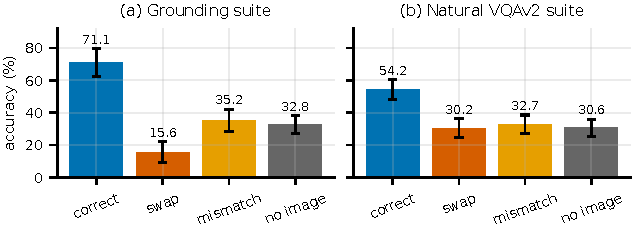
\includegraphics[width=0.62\linewidth]{figures/task2_final.pdf}
\caption{Final accuracy by image condition with 95\% intervals (196 tokens).}
\label{fig:t2-final}
\end{figure}


\paragraph{Learning curves.} Figure~\ref{fig:t2-curves} adds the training loss and the development answer NLL under the correct, partner, and no-image inputs to the curves of Figure~\ref{fig:t2-dev}. The training loss falls from about 5.5 to 2.4 during Stage 1, drops to about 0.7 when question answering is introduced, and rises briefly at the start of Stage 3 when the natural questions enter the mixture. The no-image NLL is constant in Stage 1 because only the connector is trained there, and it is not used without an image. It falls after Stage 2 and ends at 2.18 (grounding) and 2.53 (natural), above the correct-image values of 0.90 and 1.19. On the final test, a swapped image gives a higher NLL than no image in the grounding suite (3.88 against 2.04) and an equal one in the natural suite (2.44 against 2.46), so on template questions a wrong image is more harmful than no image.

\begin{figure}[H]
\centering
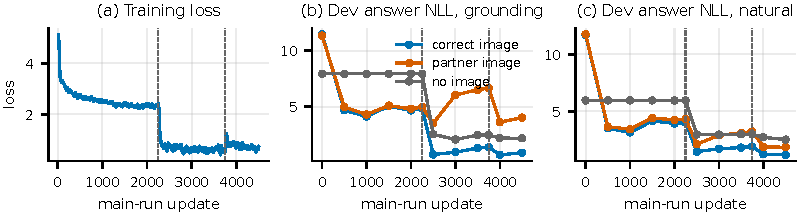
\includegraphics[width=\linewidth]{figures/task2_curves_full.pdf}
\caption{Training loss and development answer NLL for the 196-token model. Dashed lines mark the stage boundaries.}
\label{fig:t2-curves}
\end{figure}

\begin{table}[H]
\centering
\caption{Question-type accuracy (\%), empty-answer rate, and generation time per answer on the final test sets (196 tokens). The three type columns are presence, counting, and unused for grounding, and yes/no, number, and other for natural questions.}
\label{tab:t2-types}
\footnotesize
\begin{tabular}{llccccc}
\toprule
Suite & Image & Empty (\%) & s/answer & Type 1 & Type 2 & Type 3 \\
\midrule
Grounding & Correct & 0.0 & 0.038 & 93.8 & 48.4 & n/a \\
 & Swap & 0.0 & 0.040 & 6.2 & 25.0 & n/a \\
 & Mismatched & 0.0 & 0.035 & 48.4 & 21.9 & n/a \\
 & No image & 0.0 & 0.028 & 50.0 & 15.6 & n/a \\
Natural & Correct & 0.0 & 0.044 & 59.2 & 62.3 & 43.8 \\
 & Swap & 0.0 & 0.041 & 50.8 & 12.3 & 21.5 \\
 & Mismatched & 0.0 & 0.042 & 49.9 & 31.9 & 16.1 \\
 & No image & 0.0 & 0.026 & 48.6 & 24.2 & 16.9 \\
\bottomrule
\end{tabular}
\end{table}

No model output was empty under any condition. Generation without an image is faster (0.026 to 0.028 s against 0.035 to 0.044 s) because the 196 visual tokens are removed from the prefix.

\paragraph{Qualitative examples.} Figure~\ref{fig:t2-qual} shows eight aligned complementary pairs chosen by a fixed rule: in each suite and bucket, the first two pairs in sorted pair-ID order. The buckets are ``image driven'' (both correct-image answers match the references and both swapped answers equal the partner's reference) and ``wrong with correct image'' (at least one wrong answer). No grounding pair produced unchanged predictions under the swap, so that bucket is empty. In the image-driven pairs the answers move with the image (trucks: 2 and 1 become 1 and 2 under the swap; giraffes: 4 and 1 become 1 and 4). In the failures the answer often does not depend on the image: the model answers 3 for both kitchens (references 3 and 1), ``orange'' for both ring photos (references gold and silver), and ``yes'' for both vase photos (references no and yes). In the bowls pair it counts 1 and 3 instead of 1 and 4, and under the swap each image receives the partner's count.\par\medskip

\begin{figure}[H]
\centering
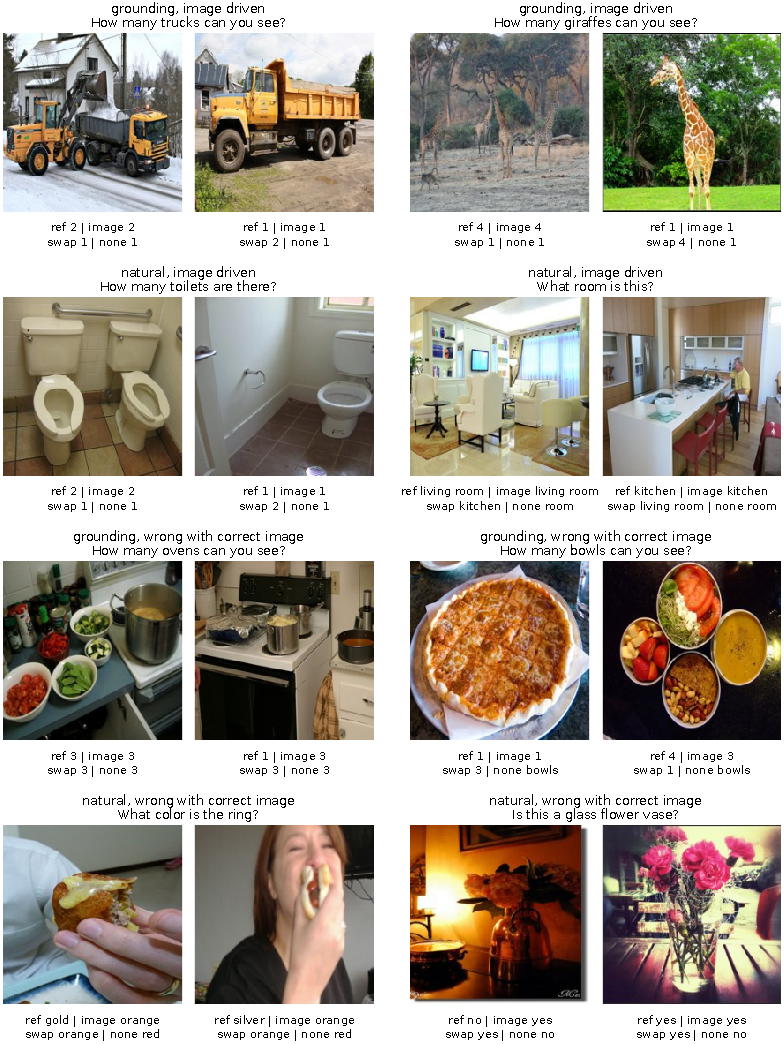
\includegraphics[width=0.82\linewidth]{figures/task2_qualitative.pdf}
\caption{Aligned examples. Below each image: the reference, the prediction with that image, with the partner image (swap), and with no image. Rows 1 and 2 are image driven and rows 3 and 4 are failures.}
\label{fig:t2-qual}
\end{figure}

\paragraph{Optional 49-token run.} The 49-token model uses the same seed, data, budgets, and evaluation, with a new connector and adapters. Table~\ref{tab:t2-49} compares the two runs.

\begin{table}[H]
\centering
\caption{196 against 49 visual tokens (final test, 95\% intervals). Swap advantage is the accuracy with the correct image minus that with the swap, in points.}
\label{tab:t2-49}
\footnotesize
\begin{tabular}{lcccccc}
\toprule
Tokens & Suite & Accuracy (\%) & Pair acc. (\%) & Swap advantage & s/answer & Train time (s) \\
\midrule
196 & Grounding & 71.1 [62.5, 79.7] & 56.2 & 55.5 [41.4, 69.5] & 0.038 & 5,701 \\
49 & Grounding & 68.8 [59.4, 77.3] & 53.1 & 57.0 [44.5, 68.8] & 0.023 & 3,218 \\
196 & Natural & 54.2 [48.1, 60.3] & 19.8 & 24.0 [15.3, 32.9] & 0.044 & (same run) \\
49 & Natural & 47.6 [40.4, 54.8] & 20.8 & 16.6 [6.6, 26.9] & 0.033 & (same run) \\
\bottomrule
\end{tabular}
\end{table}

\paragraph{Training note.} The gradient scaler skipped the first 5 updates of the 196-token run and the first 4 of the 49-token run while it lowered its initial scale, so the connector gradient norm recorded at update 1 in \texttt{sanity.json} is not finite. All later updates were finite and the loss decreased, which shows that gradients reach the connector. No backbone parameter received a gradient.

\section{Supplementary Results for Task 3}
\label{app:t3}
Table~\ref{tab:app-signals} reports within-question associations at $N=32$ on held-out questions with both correct and incorrect rollouts (469 on MATH, 640 on MathVista). Top-bottom is the difference in correctness between the highest and lowest quartile of rollouts by the signal within a question, averaged over questions. Top-1 is the accuracy of selecting the highest-scoring rollout. The MathVista gold labels in the export are option letters while the question metadata gives the choice text; all 525 mismatches between the two were of this kind in multiple-choice questions, so our grading, which converts both to letters, is not affected. The first-rollout accuracy of the supplied MathVista rollouts is 54.1\% under our grading, with 9.5\% of rollouts without an extractable answer, so the scores are not directly comparable with published MathVista results.

\begin{table}[H]
\centering
\caption{Within-question signal analysis at $N=32$ (held-out), with bootstrap intervals for the top-bottom difference.}
\label{tab:app-signals}
\footnotesize
\begin{tabular}{llccc}
\toprule
Data & Signal & Spearman with correctness & Top-bottom quartile (pp) & Top-1 accuracy (\%) \\
\midrule
MATH & Length (tokens) & -0.077 & -7.8 [-10.8, -5.0] & 54.3 \\
 & Mean log-probability & 0.134 & 13.4 [10.8, 15.8] & 64.1 \\
 & Self-certainty & 0.199 & 20.5 [17.9, 23.2] & 70.8 \\
 & Shortest rollout & 0.077 & 7.9 [5.1, 10.4] & 62.6 \\
MathVista & Length (tokens) & -0.043 & -4.5 [-6.7, -2.1] & 45.4 \\
 & Mean log-probability & 0.034 & 2.5 [0.3, 4.6] & 49.0 \\
 & Self-certainty & 0.050 & 4.6 [2.4, 6.7] & 55.6 \\
 & Vision engagement & 0.035 & 4.2 [2.1, 6.6] & 54.3 \\
 & VisConf & 0.086 & 9.0 [6.7, 11.3] & 58.5 \\
 & VisConf, token-wise & 0.077 & 8.7 [6.3, 10.9] & 56.9 \\
 & Shortest rollout & 0.043 & 4.3 [2.3, 6.5] & 53.9 \\
\bottomrule
\end{tabular}
\end{table}


\paragraph{Illustrative trajectories.} Figure~\ref{fig:t3-traj} shows the token-level calibrated confidence $c_t$ and visual engagement $v_t$ for the rollouts with the highest and the lowest VisConf score in three held-out MathVista questions. The rule is to take the first held-out questions, in the permuted order, for which (a) the SC answer and the top-VisConf rollout are both correct (question 99), (b) the top-VisConf rollout is wrong and SC is correct (question 379), and (c) the top-VisConf rollout is correct and SC is wrong (question 893). Three observations hold in all three cases. First, $v_t$ is largest within the first 10 to 40 generated tokens and then decays to about 0.02, so the rollout mean $V_i$ is larger for short rollouts. Second, the highest-VisConf rollout is the shorter one (92, 116, and 92 tokens against 160, 197, and 213 for the lowest). Third, $c_t$ varies much more within a rollout (roughly 0.1 to 0.8) than $v_t$ does after the first tokens, so rollout-level means hide most of the token-level structure. In case (b) the top-VisConf rollout answers B with a mean confidence of 0.39 and a mean engagement of 0.06, the same range as the correct rollout of case (c), so neither signal separates correct from wrong on its own.

\begin{figure}[H]
\centering
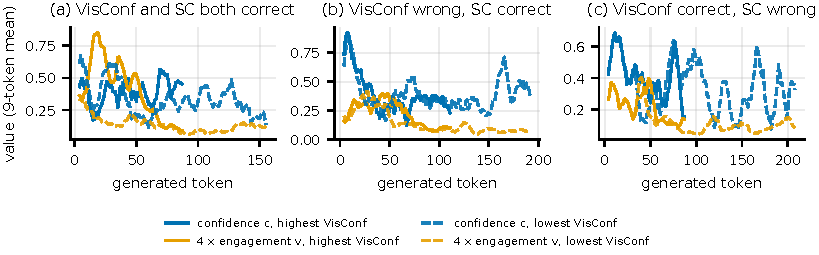
\includegraphics[width=\linewidth]{figures/task3_trajectories.pdf}
\caption{Calibrated confidence $c_t$ and visual engagement $v_t$ (scaled by 4 for visibility) along the highest-VisConf (solid) and lowest-VisConf (dashed) rollouts of three held-out MathVista questions.}
\label{fig:t3-traj}
\end{figure}

\paragraph{Illustrative cases.} Table~\ref{tab:t3-cases} lists cases chosen by stated rules. Selection cases are the first held-out questions in the permuted order, for the first reveal order and $N=32$, grouped by disagreement type. Refinement cases are the first live questions whose correctness changed after review. Premature stops are the first held-out questions for which the quality-aware rule stopped with an incorrect answer while fixed-32 SC was correct. Two selection cases are ties: when two answers have equal support, SC returns the one from the earlier rollout, and the outcome depends on the reveal order, while RWC can break the tie with the score. In the other two selection cases the plurality answer, which is correct, is overturned by the score ranking (self-certainty or VisConf). The case with a single correct rollout out of 32 shows a sampling failure that no selector can repair.

\begin{table}[H]
\centering
\caption{Illustrative cases. Counts are the number of the 32 rollouts supporting an answer. MV: MathVista; NA: NO\_ANSWER.}
\label{tab:t3-cases}
\footnotesize
\begin{tabular}{p{2.7cm}lp{7.3cm}}
\toprule
Case & Question & Observation \\
\midrule
SC right, score wrong & MATH 3157 (gold 4) & Counts 4: 11, 1: 10, 0: 10. SC returns 4, self-certainty RWC returns 0. \\
SC right, score wrong & MV 552 (gold 4) & Counts 4: 14, 3: 9, 2: 9. SC returns 4, VisConf RWC returns 2. \\
Score right, SC wrong & MATH 2460 (gold 154) & Counts 154: 11, 58: 11, NA: 3. Tie; SC returns 58, RWC returns 154. \\
Score right, SC wrong & MV 19 (gold 400) & Counts 400: 16, 600: 16. Tie; SC returns 600, VisConf RWC returns 400. \\
Sampling failure & MV 204 (gold 12) & One correct rollout; SC and VisConf RWC both return 4 (7 votes). \\
Refinement, wrong to correct & Live 3504 (gold 216) & Initial response cut at 1,024 tokens without a boxed answer; the review completes it and answers 216. \\
Refinement, wrong to correct & Live 196 (gold 81) & Same pattern: no boxed answer after 1,024 tokens; the review answers 81. \\
Refinement, correct to wrong & Live 1324 (gold 3/16) & The initial answer 3/16 is changed to 3/32 by the review. \\
Premature stop & MATH 2460, order 7 & First four candidates 154, 58, 58, 58; stop at $N=4$ with 58; the full pool has 154 and 58 at 11 votes each. \\
Premature stop & MATH 1903, order 4 & First four candidates 80, 75, 120, 75; stop with 75 ($2/4$ support); gold 80 has 7 votes, 75 has 7. \\
Premature stop & MV 552, order 4 & First four candidates 3, 2, 3, 3; stop with 3 ($3/4$); gold 4 has 14 votes in the full pool, 3 has 9. \\
\bottomrule
\end{tabular}
\end{table}

\paragraph{Adaptive stopping by pool difficulty.} Questions were grouped by the fraction of their 32 rollouts that are correct, which uses retrospective information for analysis only. For MATH under the agreement rule, questions with at least two thirds correct (476 questions) reach 99.9\% with 4.3 rollouts on average, intermediate questions (102) reach 89.0\% against 91.2\% for fixed-32 with 18.4 rollouts, and hard questions (222) reach 10.8\% against 10.0\% with 24.8 rollouts. For MathVista the three groups (354, 173, and 273 questions) reach 99.5\%, 71.3\% (fixed-32: 81.7\%), and 10.5\% (fixed-32: 5.9\%). On the hard groups the adaptive policy is above fixed-32, which may reflect chance: an early plurality over few samples is sometimes right where a later plurality over many weak answers is not.

\end{document}
